
\documentclass[11pt,compress,t,notes=noshow, xcolor=table]{beamer}
\usepackage[]{graphicx}\usepackage[]{color}
% maxwidth is the original width if it is less than linewidth
% otherwise use linewidth (to make sure the graphics do not exceed the margin)
\makeatletter
\def\maxwidth{ %
  \ifdim\Gin@nat@width>\linewidth
    \linewidth
  \else
    \Gin@nat@width
  \fi
}
\makeatother

\definecolor{fgcolor}{rgb}{0.345, 0.345, 0.345}
\newcommand{\hlnum}[1]{\textcolor[rgb]{0.686,0.059,0.569}{#1}}%
\newcommand{\hlstr}[1]{\textcolor[rgb]{0.192,0.494,0.8}{#1}}%
\newcommand{\hlcom}[1]{\textcolor[rgb]{0.678,0.584,0.686}{\textit{#1}}}%
\newcommand{\hlopt}[1]{\textcolor[rgb]{0,0,0}{#1}}%
\newcommand{\hlstd}[1]{\textcolor[rgb]{0.345,0.345,0.345}{#1}}%
\newcommand{\hlkwa}[1]{\textcolor[rgb]{0.161,0.373,0.58}{\textbf{#1}}}%
\newcommand{\hlkwb}[1]{\textcolor[rgb]{0.69,0.353,0.396}{#1}}%
\newcommand{\hlkwc}[1]{\textcolor[rgb]{0.333,0.667,0.333}{#1}}%
\newcommand{\hlkwd}[1]{\textcolor[rgb]{0.737,0.353,0.396}{\textbf{#1}}}%
\let\hlipl\hlkwb

\usepackage{framed}
\makeatletter
\newenvironment{kframe}{%
 \def\at@end@of@kframe{}%
 \ifinner\ifhmode%
  \def\at@end@of@kframe{\end{minipage}}%
  \begin{minipage}{\columnwidth}%
 \fi\fi%
 \def\FrameCommand##1{\hskip\@totalleftmargin \hskip-\fboxsep
 \colorbox{shadecolor}{##1}\hskip-\fboxsep
     % There is no \\@totalrightmargin, so:
     \hskip-\linewidth \hskip-\@totalleftmargin \hskip\columnwidth}%
 \MakeFramed {\advance\hsize-\width
   \@totalleftmargin\z@ \linewidth\hsize
   \@setminipage}}%
 {\par\unskip\endMakeFramed%
 \at@end@of@kframe}
\makeatother

\definecolor{shadecolor}{rgb}{.97, .97, .97}
\definecolor{messagecolor}{rgb}{0, 0, 0}
\definecolor{warningcolor}{rgb}{1, 0, 1}
\definecolor{errorcolor}{rgb}{1, 0, 0}
\newenvironment{knitrout}{}{} % an empty environment to be redefined in TeX

\usepackage{alltt}
\newcommand{\SweaveOpts}[1]{}  % do not interfere with LaTeX
\newcommand{\SweaveInput}[1]{} % because they are not real TeX commands
\newcommand{\Sexpr}[1]{}       % will only be parsed by R
\newcommand{\xmark}{\ding{55}}%


\usepackage[english]{babel}
\usepackage[utf8]{inputenc}

\usepackage{dsfont}
\usepackage{verbatim}
\usepackage{amsmath}
\usepackage{amsfonts}
\usepackage{amssymb}
\usepackage{bm}
\usepackage{csquotes}
\usepackage{multirow}
\usepackage{longtable}
\usepackage{booktabs}
\usepackage{enumerate}
\usepackage[absolute,overlay]{textpos}
\usepackage{psfrag}
\usepackage{algorithm}
\usepackage{algpseudocode}
\usepackage{eqnarray}
\usepackage{arydshln}
\usepackage{tabularx}
\usepackage{placeins}
\usepackage{tikz}
\usepackage{setspace}
\usepackage{colortbl}
\usepackage{mathtools}
\usepackage{wrapfig}
\usepackage{bm}
\usepackage{amsmath}
\usepackage{pifont}
\usepackage{xcolor} %colored math symbols

\usetikzlibrary{shapes,arrows,automata,positioning,calc,chains,trees, shadows}
\tikzset{
  %Define standard arrow tip
  >=stealth',
  %Define style for boxes
  punkt/.style={
    rectangle,
    rounded corners,
    draw=black, very thick,
    text width=6.5em,
    minimum height=2em,
    text centered},
  % Define arrow style
  pil/.style={
    ->,
    thick,
    shorten <=2pt,
    shorten >=2pt,}
}

\usepackage{subfig}

% Defines macros and environments
\usepackage{../../style/lmu-lecture}


\let\code=\texttt
\let\proglang=\textsf

\setkeys{Gin}{width=0.9\textwidth}

\setbeamertemplate{frametitle}{\expandafter\uppercase\expandafter\insertframetitle}

\usepackage{bbm}
% basic latex stuff
\newcommand{\pkg}[1]{{\fontseries{b}\selectfont #1}} %fontstyle for R packages
\newcommand{\lz}{\vspace{0.5cm}} %vertical space
\newcommand{\dlz}{\vspace{1cm}} %double vertical space
\newcommand{\oneliner}[1] % Oneliner for important statements
{\begin{block}{}\begin{center}\begin{Large}#1\end{Large}\end{center}\end{block}}


%new environments
\newenvironment{vbframe}  %frame with breaks and verbatim
{
 \begin{frame}[containsverbatim,allowframebreaks]
}
{
\end{frame}
}

\newenvironment{vframe}  %frame with verbatim without breaks (to avoid numbering one slided frames)
{
 \begin{frame}[containsverbatim]
}
{
\end{frame}
}

\newenvironment{blocki}[1]   % itemize block
{
 \begin{block}{#1}\begin{itemize}
}
{
\end{itemize}\end{block}
}

\newenvironment{fragileframe}[2]{  %fragile frame with framebreaks
\begin{frame}[allowframebreaks, fragile, environment = fragileframe]
\frametitle{#1}
#2}
{\end{frame}}


\newcommand{\myframe}[2]{  %short for frame with framebreaks
\begin{frame}[allowframebreaks]
\frametitle{#1}
#2
\end{frame}}

\newcommand{\remark}[1]{
  \textbf{Remark:} #1
}


\newenvironment{deleteframe}
{
\begingroup
\usebackgroundtemplate{
\includegraphics[width=\paperwidth,height=\paperheight]{../style/color/red.png}}
 \begin{frame}
}
{
\end{frame}
\endgroup
}
\newenvironment{simplifyframe}
{
\begingroup
\usebackgroundtemplate{
\includegraphics[width=\paperwidth,height=\paperheight]{../style/color/yellow.png}}
 \begin{frame}
}
{
\end{frame}
\endgroup
}\newenvironment{draftframe}
{
\begingroup
\usebackgroundtemplate{
\includegraphics[width=\paperwidth,height=\paperheight]{../style/color/green.jpg}}
 \begin{frame}
}
{
\end{frame}
\endgroup
}
% https://tex.stackexchange.com/a/261480: textcolor that works in mathmode
\makeatletter
\renewcommand*{\@textcolor}[3]{%
  \protect\leavevmode
  \begingroup
    \color#1{#2}#3%
  \endgroup
}
\makeatother


\input{../../latex-math/basic-math}
\input{../../latex-math/basic-ml}
\input{../../latex-math/ml-nn}

\newcommand{\titlefigure}{plots/05_conv_variations/3d/3dconv.png}
%modify picture
\newcommand{\learninggoals}{
  \item 1D Convolutions
  \item 2D Convolutions
  \item 3D Convolutions
}

\title{Deep Learning}
\date{}



\begin{document}

\lecturechapter{1D / 2D / 3D Convolutions}
\lecture{I2DL}

\begin{frame} {Common Machine Vision Tasks}
  \begin{itemize}
    \item Image Classification: Assign a \textit{single} label to the whole image.
    \item Object localization / detection: Draw \textbf{bounding boxes} around (and classify) one or more objects in the image.
    \item Semantic Segmentation: The goal here is to draw \textbf{outlines} between classes \textit{without} differentiating between different instances of a given class.
    \item Instance segmentation: This is a hybrid of the previous two tasks. The goal is to classify \textit{each} object in the image and draw a \textit{separate} outline around it.
    \item Note: This is not an exhaustive list. There are \textit{many} others.
    \end{itemize}
\end{frame}


\begin{frame} {Common Machine Vision Tasks}
  \begin{figure}
    \centering
      \scalebox{0.90}{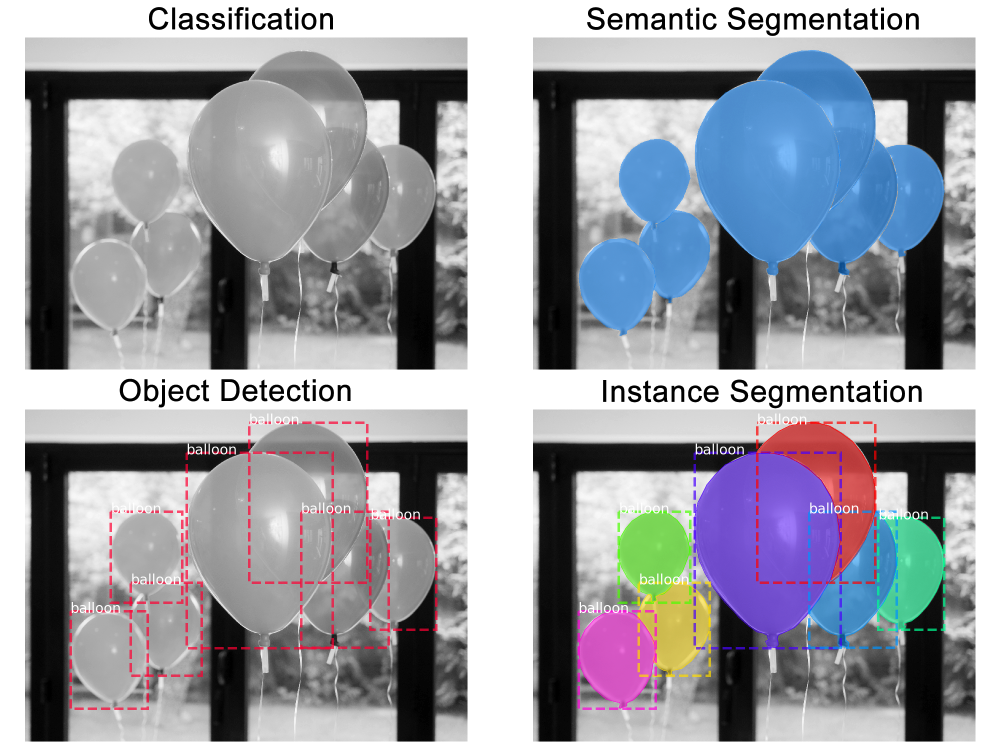
\includegraphics{plots/maskrcnn/mask_types.png}}
      \tiny{\\credit: Waleed Abulla}
  \end{figure}
    Instance segmentation is the most challenging task!
\end{frame}

\begin{frame} {Mask R-CNN - Overview}
  \begin{itemize}
    \item Mask R-CNN (He et al., 2017) belongs to an important class of CNNs known as Region-based CNNs (or R-CNNs).
    \item It extends the Faster R-CNN (Ren et al., 2015) architecture (which performs classification and detection) by adding a branch for segmentation (more on this later).
    \item Therefore, Mask R-CNN performs classification, detection \textit{and} instance segmentation in parallel!
    \item It was developed at Facebook in 2017 and trained using the COCO (Common Objects in Context) dataset.
    \item Note: Each training example has ground truth class labels, bounding boxes and segmentation masks.
    \item This case-study is only meant to be a 'quick tour' of Mask R-CNN. If any of the details are unclear, please read the paper.
  \end{itemize}
\end{frame}

\begin{frame} {Mask R-CNN architecture}
  \begin{figure}
    \centering
      \scalebox{0.5}{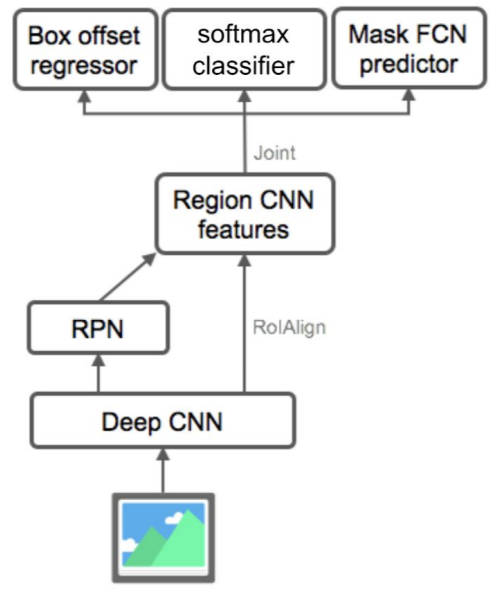
\includegraphics{plots/maskrcnn/mask_arch_2.png}}
      \tiny{\\credit: UCSD}
      \caption{Mask R-CNN architecture.}
  \end{figure}
\end{frame}

\begin{frame} {Mask R-CNN architecture}
  \begin{figure}
    \centering
      \scalebox{0.95}{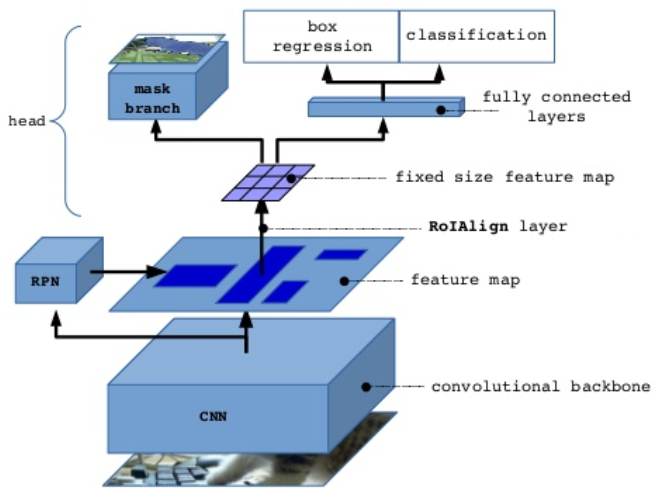
\includegraphics{plots/maskrcnn/mask_arch_1.png}}
      \tiny{\\credit: Georgia Gkioxari}
      \caption{Mask R-CNN architecture.}
  \end{figure}
\end{frame}

\begin{frame} {Mask R-CNN architecture - Stage One}
  \begin{figure}
    \centering
      \scalebox{0.95}{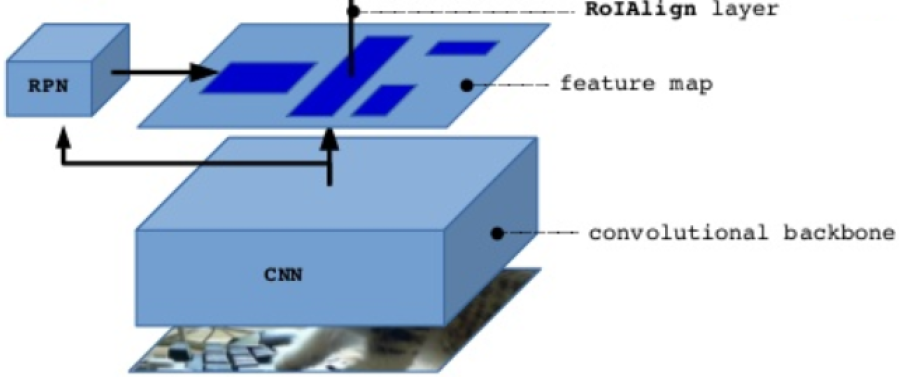
\includegraphics{plots/maskrcnn/mask_stage1.png}}
  \end{figure}
  \begin{itemize}
    \item \textit{Stage One}: Consists of a "backbone" network and a Region Proposal Network (RPN).
    \item The backbone network extracts the feature maps from an image and the RPN identifies promising regions, or Regions of Interest (ROIs) that might contain interesting objects.
    \item The ROIAlign layer then resizes the ROIs so that they all have the same spatial dimensions.
  \end{itemize}
\end{frame}

\begin{frame} {Mask R-CNN architecture - Stage Two}
  \begin{figure}
    \centering
      \scalebox{0.95}{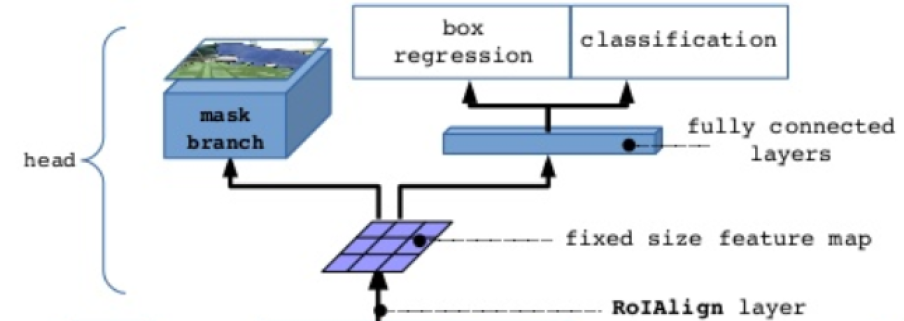
\includegraphics{plots/maskrcnn/mask_stage2.png}}
  \end{figure}
  \begin{itemize}
    \item The resized ROIs are then fed to the \textit{Stage Two} network (pictured above).
    \item This has three branches: one each for classification, detection/localization and segmentation.
  \end{itemize}
\end{frame}

\begin{frame} {Stage One - Backbone}
  \begin{itemize}
    \item The backbone architecture can be based on any generic CNN.
    \item In the paper, the authors implement Mask R-CNN using ResNet.
    \item ResNets are divided into 5 "stages" where each stage consists of several convolutional layers.
    \item The authors use the first 4 stages of ResNet-50 or ResNet-101 as the backbone network.
    %\item The output of the 4th stage , which is $14 \times 14 \times 1024$ , will now serve as the input to the Region Proposal Network.
    \item The output of the backbone network will now serve as the input to the Region Proposal Network.
  \end{itemize}
\end{frame}

\begin{frame} {Stage One - Region Proposal Network}
  \begin{itemize}
    \item Lightweight network that works directly on the final feature map generated by the backbone network.
    \item Consists of a $3 \times 3$ convolutional layer and $1 \times 1$ convolutional layers.
    \item The RPN looks at small $n \times n$ regions of the input feature map (n = 3, in our case).
    \item At \textbf{each} such location, the RPN simultaneously proposes multiple regions of interest (ROIs) that might contain objects.
    \item In order to accomplish this, each such $n \times n$ region is associated with $k$ \textbf{anchor boxes}.
    \item The number of anchor boxes and their locations, sizes and aspect ratios are all hyperparameters.
  \end{itemize}
\end{frame}

\begin{frame} {Anchor boxes}
  \begin{figure}
    \centering
      \scalebox{0.75}{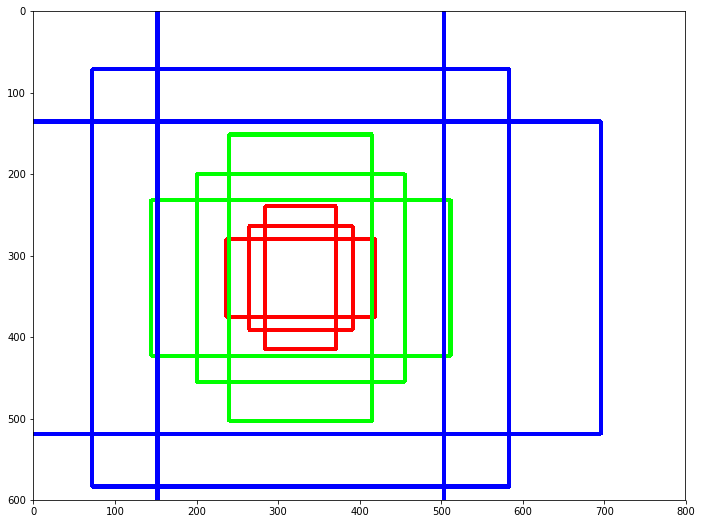
\includegraphics{plots/maskrcnn/mask_anchors.png}}
      \tiny{\\credit: Hao Gao}
      \caption{An example set of anchor boxes in a 600x800 pixel image. Three colors represent three scales or sizes: 128x128, 256x256, 512x512. For a given color, the three boxes correspond to height:width ratios of 1:1, 1:2 and 2:1. }
  \end{figure}
\end{frame}

\begin{frame} {Stage One - Region Proposal Network}
  \begin{figure}
    \centering
      \scalebox{0.7}{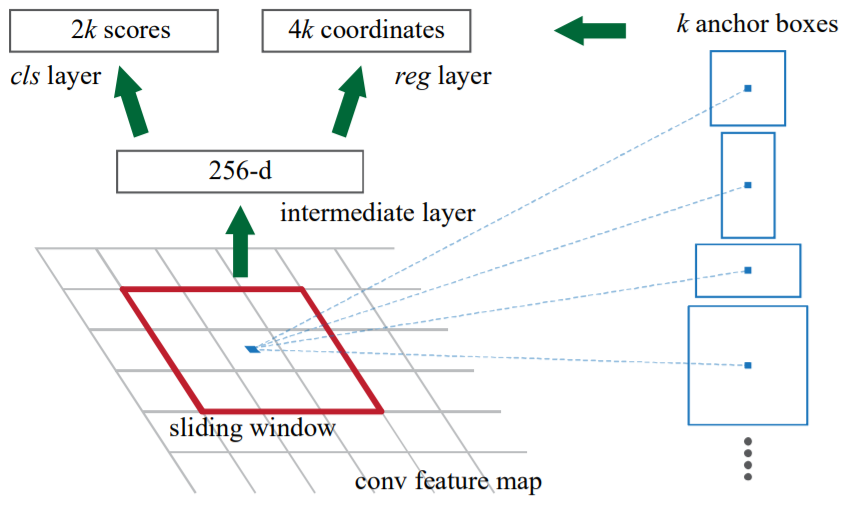
\includegraphics{plots/maskrcnn/mask_rpn.png}}
  \end{figure}
  \begin{itemize}
      \item Every location/'sliding window' in the final feature map is associated with $k = 15$ anchor boxes of varying sizes and aspect ratios.
      \item For a convolutional feature map of size $W \times H$, there will be $W \times H \times k$ anchor boxes.
      \item Cross-boundary anchors are ignored during training.
    \end{itemize}
\end{frame}

\begin{frame} {Stage One - Region Proposal Network}
  \begin{figure}
    \centering
      \scalebox{0.7}{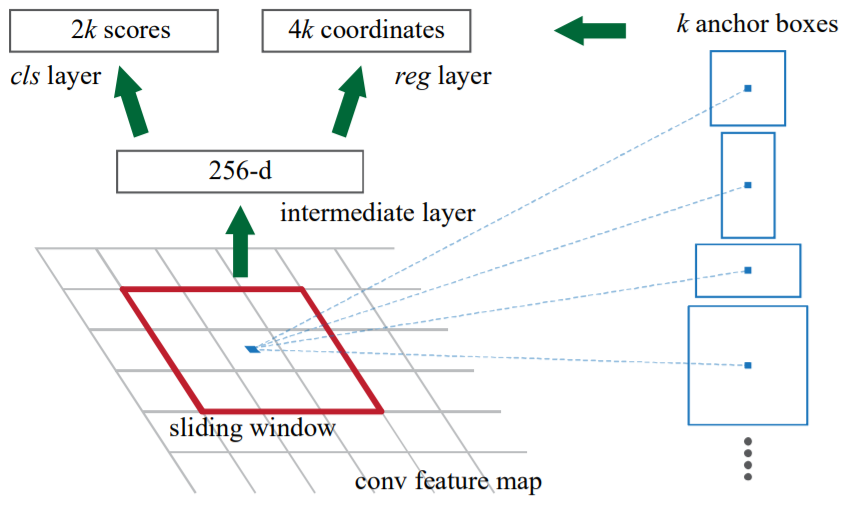
\includegraphics{plots/maskrcnn/mask_rpn.png}}
  \end{figure}
  \begin{itemize}
    \item The classifier ('cls' layer) is a dense layer which outputs $2k$ scores (to which a softmax is applied) indicating the probability of an object being present or \textit{not} present in each of the $k$ anchor boxes. 
    \item Of course, it's also possible to simply output $k$ scores (to which a logistic sigmoid is applied) instead indicating simply whether an object is present.
  \end{itemize}
\end{frame}

\begin{frame} {Stage One - Region Proposal Network}
  \begin{figure}
    \centering
      \scalebox{0.7}{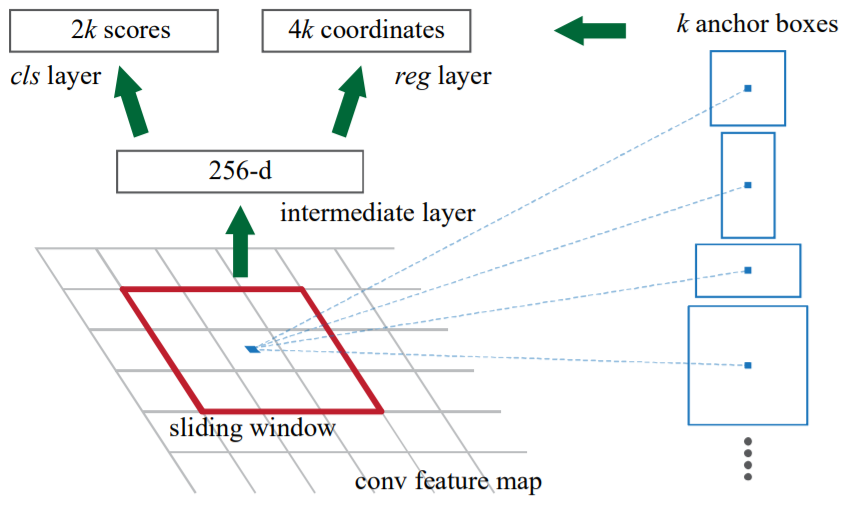
\includegraphics{plots/maskrcnn/mask_rpn.png}}
  \end{figure}
  \begin{itemize}
    \item The regression ('reg') layer is a dense layer which outputs $4k$ outputs encoding the 4 coordinates of the $k$ region proposals.
    \item These four values represent the \textit{offsets} to the location of the upper-left corner and the height and width of a (preconfigured, rectangular) anchor box.
  \end{itemize}
\end{frame}


\begin{frame} {ROI Pooling}
  \begin{itemize}
    \item The RPN has its own loss function and can be trained either separately or jointly with the rest of the network. 
    \item Stage One was computing the region proposals. Once we have have them, we enter Stage Two.
    \item Only the most promising region proposals are chosen for Stage Two using a technique called 'non-max suppression'.
    \item Please read the paper for details.
  \end{itemize}
\end{frame}

\begin{frame} {ROI Pooling}
  \begin{itemize}
    \item The region proposals are in pixel space, not feature space. Therefore, a region of the output feature map (of the backbone network) which roughly corresponds to the region proposal must first be computed.
    \item These computed regions in the feature map will be of different sizes and aspect ratios. However, the Stage Two network expects a fixed size input.
    \item Therefore, these regions (in the feature map) must then be \textit{reshaped} so that they all have the same size.
  \end{itemize}
\end{frame}

\begin{frame} {ROI Pooling}
  \begin{figure}
    \centering
      \scalebox{0.65}{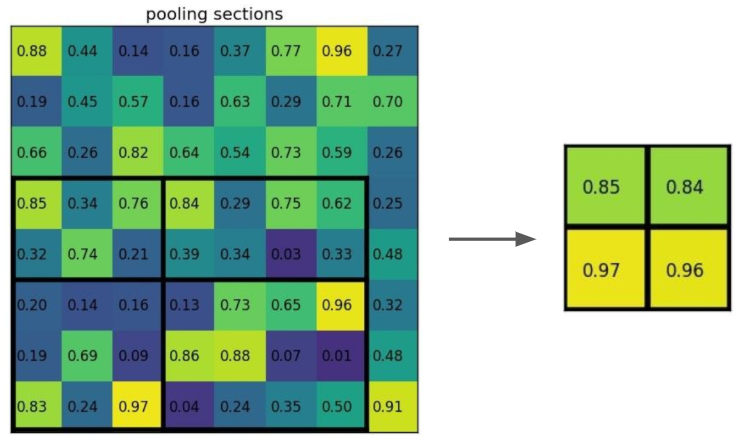
\includegraphics{plots/maskrcnn/mask_roipool.png}}
      \tiny{\\credit: deepsense.ai}
      \caption{A rectangular piece of the feature map which roughly corresponds to a region proposal is further subdivided into four unequal sections.}
  \end{figure}
  \begin{itemize}
    \item \small{To reshape, one option is to divide each rectangular region into unequal sections and perform max-pooling in each section. This is called ROIPool.
    \item However, the authors implement a more sophisticated method called ROIAlign to perform the reshaping.}
  \end{itemize}
\end{frame}

\begin{frame} {Stage Two}
  \begin{figure}
    \centering
      \scalebox{0.5}{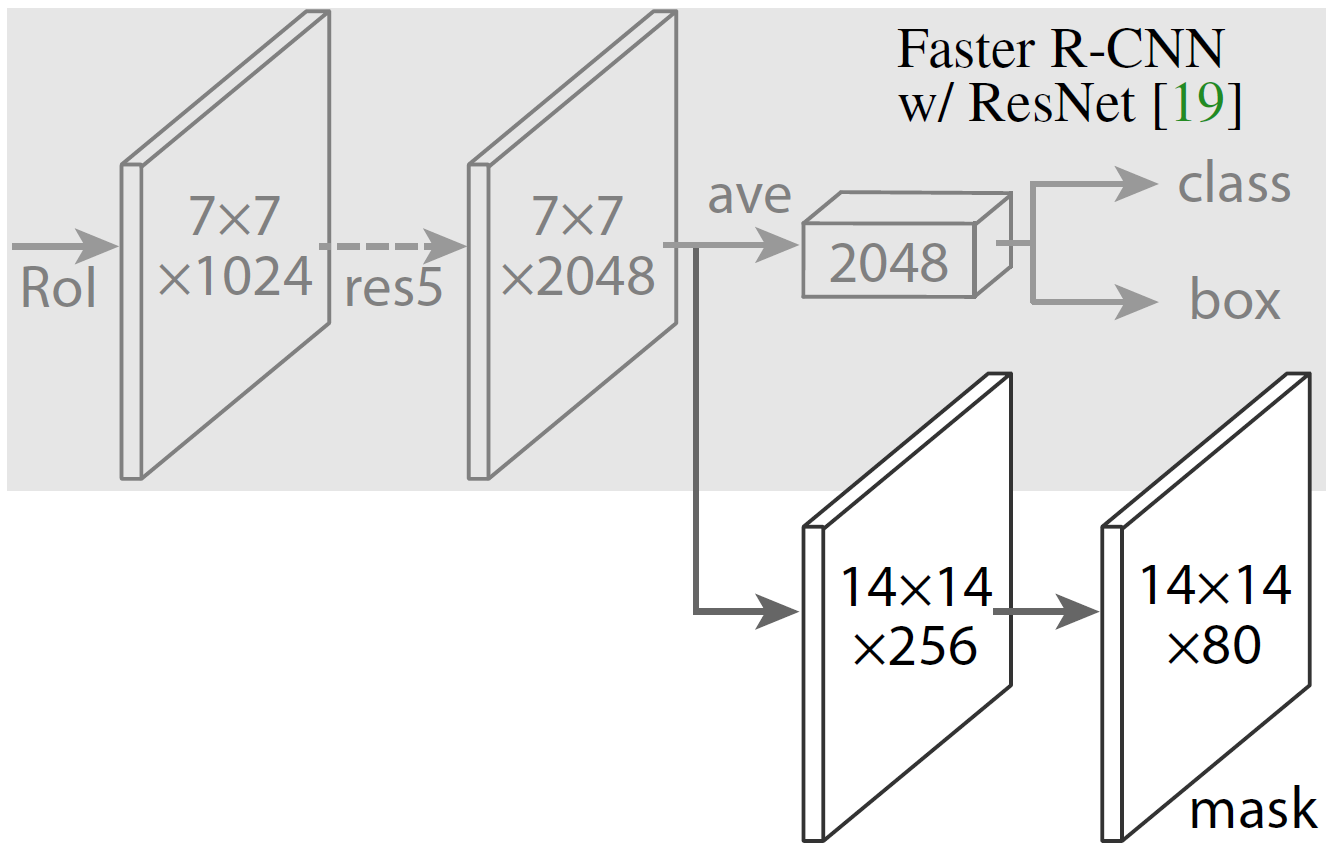
\includegraphics{plots/maskrcnn/mask_head.png}}
      \caption{\footnotesize{The three "heads" for classification ('class'), bounding box regression ('box) and instance segmentation ('mask'). The first two heads are also present in the Faster-RCNN architecture from which Mask R-CNN is derived.}
}
  \end{figure}
  \begin{itemize}
    \item After reshaping, a $7 \times 7 \times 1024$ ROI is fed to the fifth stage of ResNet ('res5') which outputs a $7 \times 7 \times 2048$ feature map.
    \item The resulting feature map is then fed to the classification, regression and mask branches.
  \end{itemize}
\end{frame}


\begin{frame} {Stage Two}
  \begin{figure}
    \centering
      \scalebox{0.5}{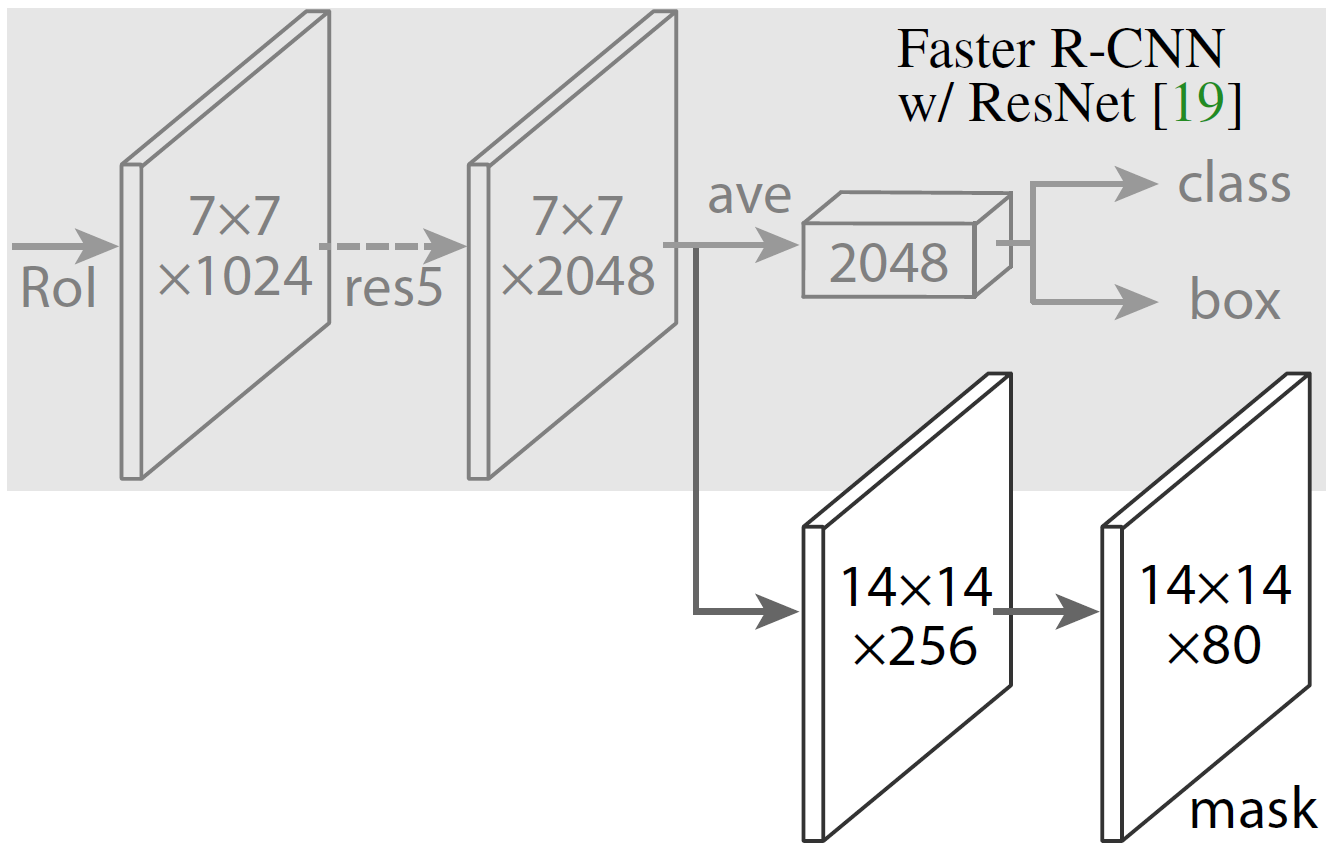
\includegraphics{plots/maskrcnn/mask_head.png}}
  \end{figure}
    \begin{itemize}
      \item \small{The $7 \times 7 \times 2048$ output of 'res5' is fed to a dense layer of size 2048.
      \item The output of the dense layer is then fed to two 'sibling' branches which contain additional dense layers.
      \item The classification head outputs a vector of length $K+1$, where $K$ is the number of classes.
      \item This vector contains the probabilities for each class and, additionally, \textit{no} class / "background" class.}
    \end{itemize}
\end{frame}

\begin{frame} {Stage Two}
  \begin{figure}
    \centering
      \scalebox{0.5}{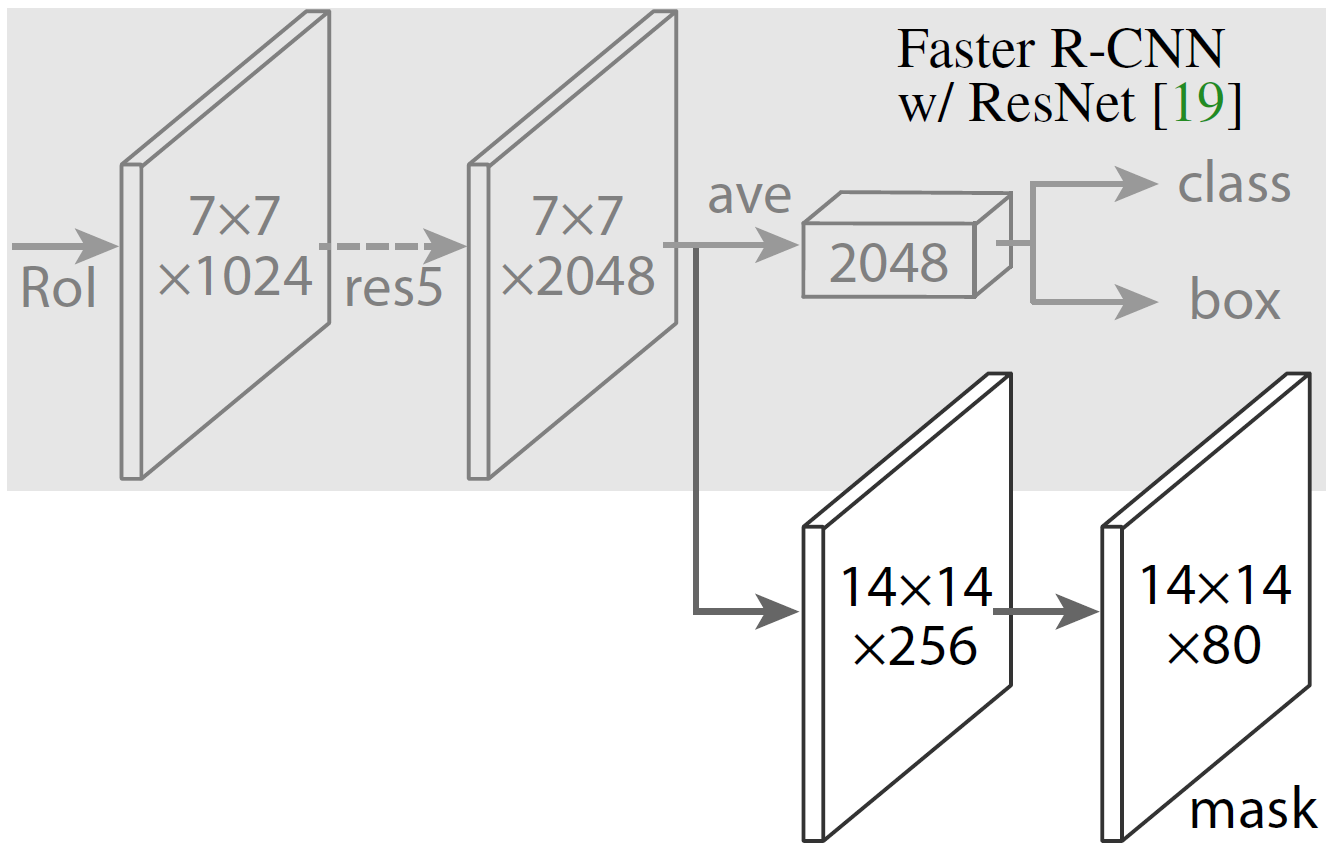
\includegraphics{plots/maskrcnn/mask_head.png}}
  \end{figure}
  \begin{itemize}
    \item The regression head outputs 4 real valued numbers for each of the $K$ classes.
    \item Each set of 4 values encodes refined bounding box predictions for one of the classes.
  \end{itemize}
\end{frame}

\begin{frame} {Stage Two}
  \begin{figure}
    \centering
      \scalebox{0.5}{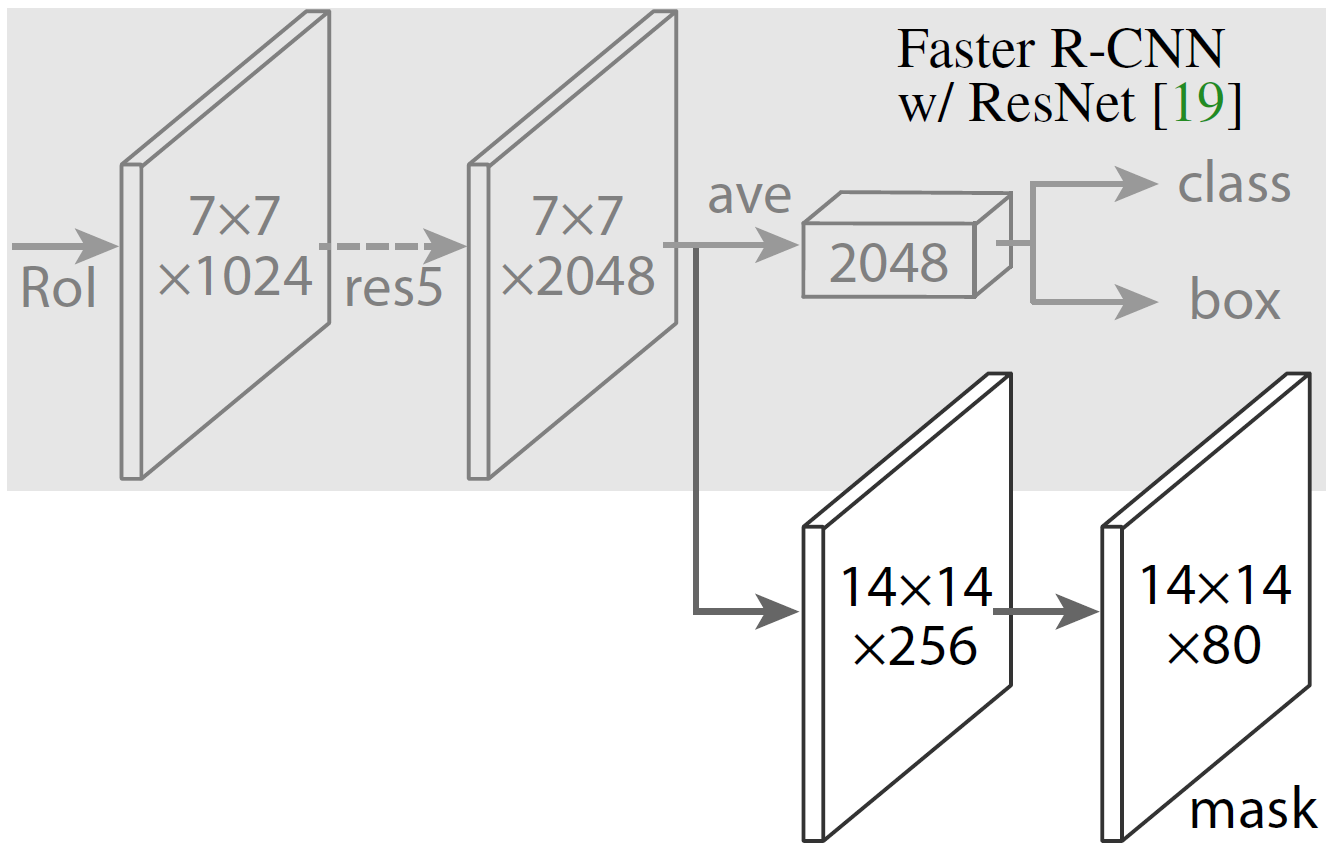
\includegraphics{plots/maskrcnn/mask_head.png}}
  \end{figure}
  \begin{itemize}
    \item \small{The segmentation head contains a transposed convolution layer which upsamples the $7 \times 7$ feature maps to $14 \times 14$.
    \item Finally, the output layer, which is a regular $1 \times 1$ convolution layer with a sigmoid activation, outputs a a $Km^2$ dimensional output ($K$ = 80 and $m$ = 14 here).
    \item This encodes $K$ masks of resolution $m \times m$, one for each class.
    \item The $m \times m$ mask is then resized to the ROI size and binarized (with a threshold of 0.5).}
  \end{itemize}
\end{frame}

\begin{frame} {Mask R-CNN - Loss Function}
  \begin{itemize}
    \item The multi-task loss function of Mask R-CNN combines the losses of the classification, localization and segmentation masks.
    \item For each ROI, the loss is $L = L_{cls} + L_{box} + L_{mask}$.
    \item $L_{cls}$ is the negative log likelihood for the true class.
    \item $L_{box}$ is a modified $L1$ loss between the predicted and true bounding box coordinates (for the true class) which is summed over the 4 values.
    \item Finally, $L_{mask}$ is the average binary cross-entropy loss.
    \item For an RoI associated with ground-truth class $k$, $L_{mask}$ is only defined on the $k$-th mask (other mask outputs do not contribute to the loss).
    \item Note: The component losses may be weighted differently.
  \end{itemize}
\end{frame}

\begin{frame} {Mask R-CNN - Training and Inference}
  \begin{itemize}
    \item Dataset: COCO ($\sim$ 100k training images).
    \item Trained on 8 GPUs with a minibatch size of 16 for 160k iterations.
    \item Learning rate: 0.02 for the first 120k, 0.002 thereafter.
    \item Weight Decay: 0.0001, Momentum: 0.9.
    \item Training time: 32 - 44 hours .
    \item Inference time: 200 ms - 400 ms on a Tesla M40.
  \end{itemize}
\end{frame}

\begin{frame} {Mask R-CNN - Examples}
   \begin{figure}
    \centering
      \scalebox{1}{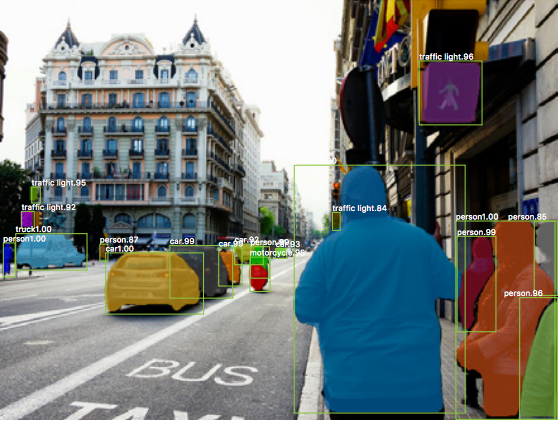
\includegraphics{plots/maskrcnn/maskrcnn.png}}
      \tiny{\\credit: He et al., 2017}
  \end{figure}
\end{frame}

\begin{frame} {Mask R-CNN - Examples}
   \begin{figure}
    \centering
      \scalebox{1}{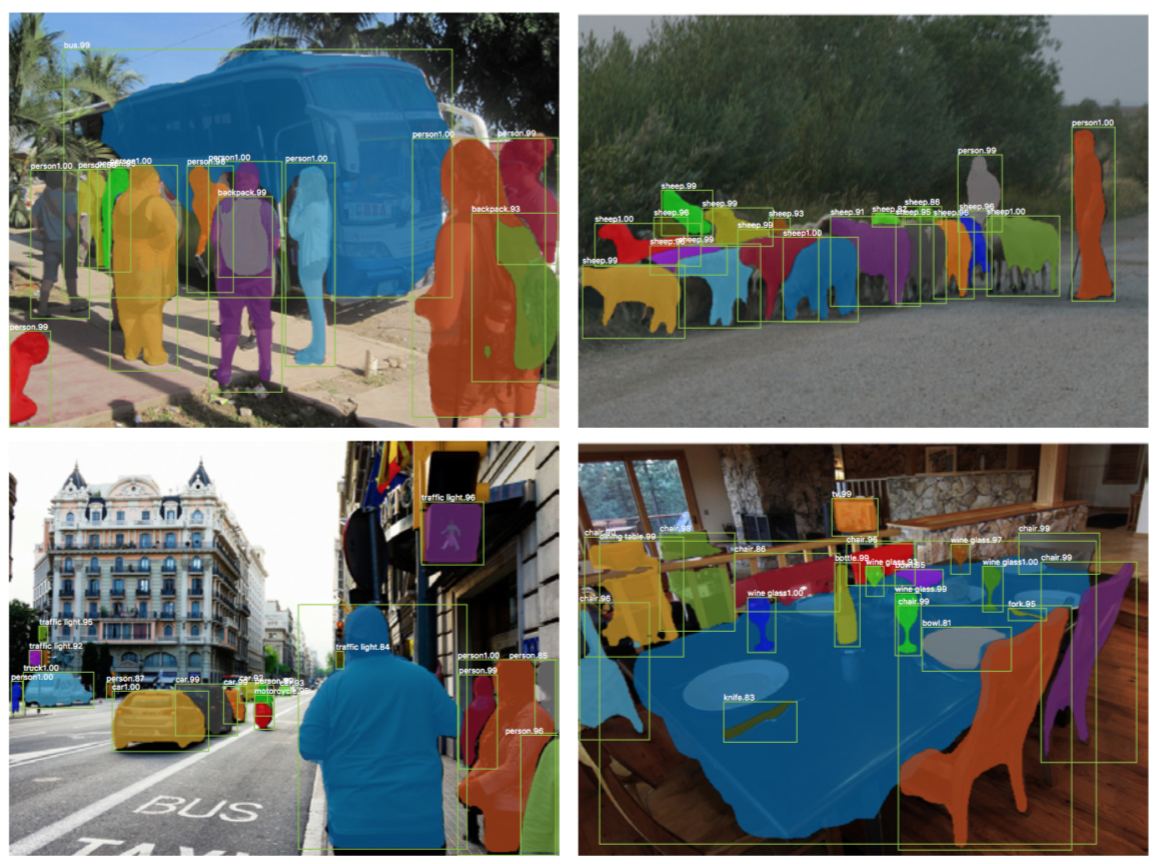
\includegraphics{plots/maskrcnn/mask_examples.png}}
      \tiny{\\credit: He et al., 2017}
  \end{figure}
\end{frame}

\begin{frame} {Mask R-CNN - Examples}
   \begin{figure}
    \centering
      \scalebox{0.90}{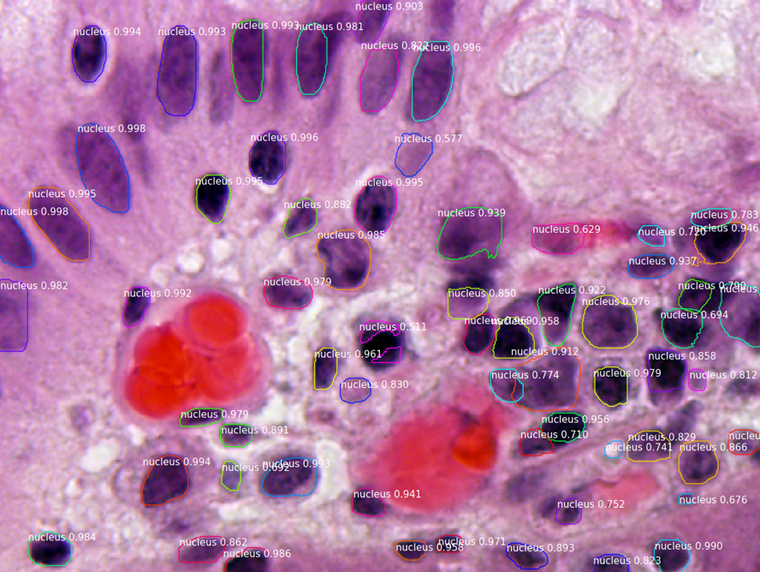
\includegraphics{plots/maskrcnn/mask_nuc.png}}
      \tiny{\\credit: Matterport}
      \caption{\footnotesize{Segmenting nuclei in microscopy images.}}
  \end{figure}
\end{frame}


% \begin{frame} {Feature Pyramid Network}
%   \begin{figure}
%     \centering
%       \scalebox{0.65}{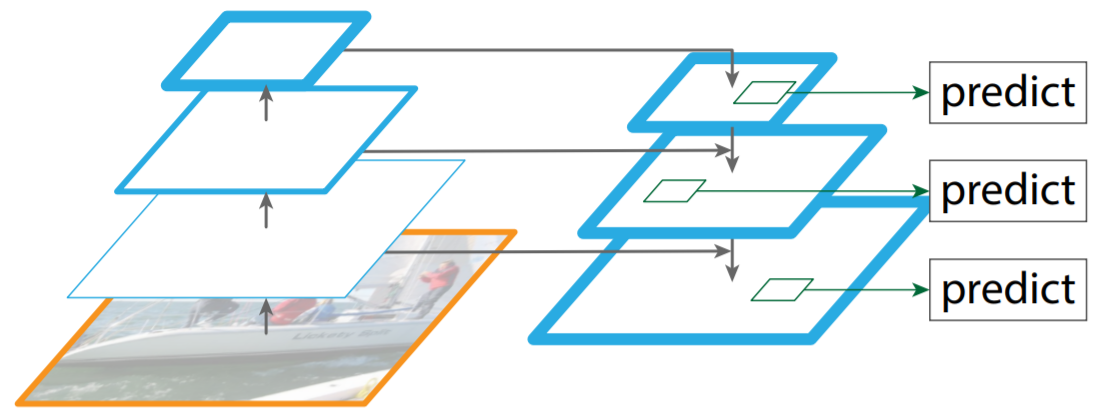
\includegraphics{plots/maskrcnn/mask_fpn0.png}}
%       \caption{Two-stage architecture (Xiang Zhang)}
%   \end{figure}
%   \begin{itemize}
%     \item Feature Pyramid Network : Resnet-101 based.
%     \item Intutions : early layers are higher resultion and layer layers capture higher level semantics. Can we get the best of both worlds?
%   \end{itemize}
% \end{frame}
% 
% \begin{frame} {Feature Pyramid Network}
%   \begin{figure}
%     \centering
%       \scalebox{0.75}{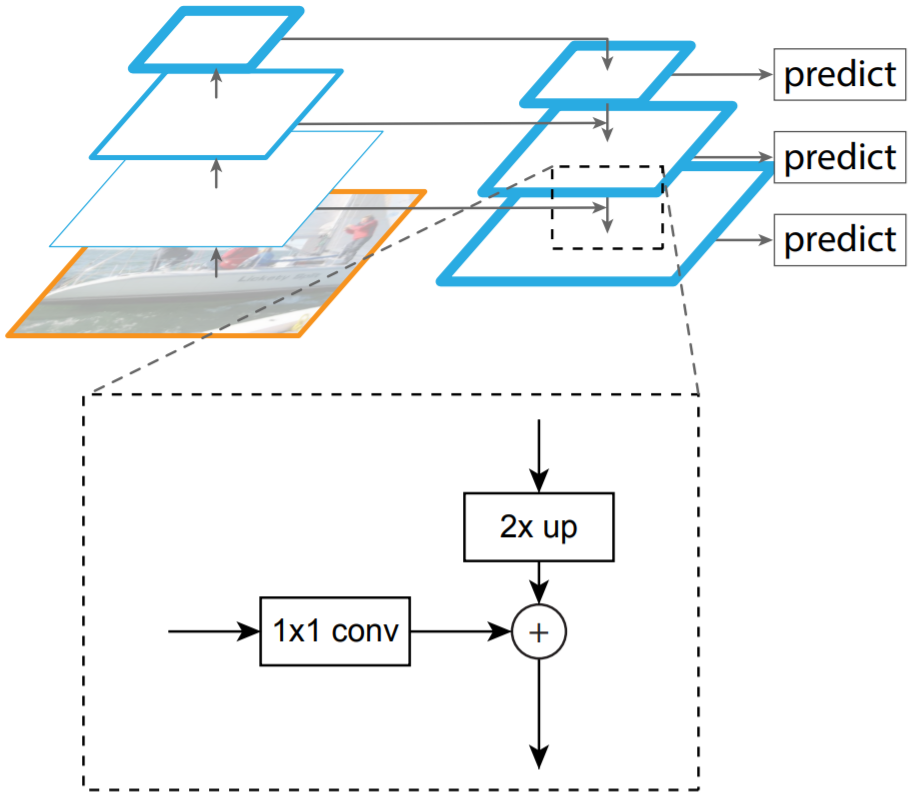
\includegraphics{plots/maskrcnn/mask_fpn.png}}
%       \caption{Two-stage architecture (Xiang Zhang)}
%   \end{figure}
% \end{frame}
% 
% \begin{frame} {Feature Pyramid Network}
%   \begin{figure}
%     \centering
%       \scalebox{0.75}{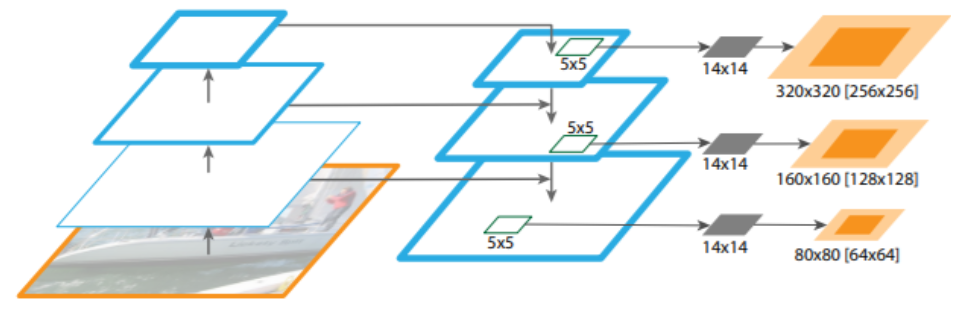
\includegraphics{plots/maskrcnn/mask_fpn2.png}}
%       \caption{Two-stage architecture (Xiang Zhang)}
%   \end{figure}
% \end{frame}






%%%%%%%%%%%%%%%%%%%%%%%%%%%%%%%%%%%%%%%%%%%%%%%%%%%%%%%%%%%%%%%%%%
%%%%%%%%%%%%%%%%%%%%%%%%%%%%%%%%%%%%%%%%%%%%%%%%%%%%%%%%%%%%%%%%%%
%%%%%%%%%%%%%%%%%%          REFERENCES          %%%%%%%%%%%%%%%%%%
%%%%%%%%%%%%%%%%%%%%%%%%%%%%%%%%%%%%%%%%%%%%%%%%%%%%%%%%%%%%%%%%%%
\begin{vbframe}
\frametitle{References}
\footnotesize{
\begin{thebibliography}{99}

%%%%%%%%%%%%%%%%%%%%%%%%%%%%%%%%%
\bibitem[Ren et al., 2015]{36} Shaoqing Ren, Kaiming He, Ross Girshick, Jian Sun (2015)
\newblock Faster R-CNN: Towards Real-Time Object Detection with Region Proposal Networks
\newblock \emph{\url{https://arxiv.org/abs/1506.01497}}
%%%%%%%%%%%%%%%%%%%%%%%%%%%%%%%%%%
%%%%%%%%%%%%%%%%%%%%%%%%%%%%%%%%%%
\bibitem[He et al., 2014]{37} Kaiming He, Georgia Gkioxari, Piotr Dollar, Ross Girshick (2017)
\newblock Mask R-CNN
\newblock \emph{\url{https://arxiv.org/abs/1703.06870}}


\end{thebibliography}
}
\end{vbframe}
%%%%%%%%%%%%%%%%%%%%%%%%%%%%%%%%%%%%%%%%%%%%%%%%%%%%%%%%%%%%%%%%%%
%%%%%%%%%%%%%%%%%%%%%%%%%%%%%%%%%%%%%%%%%%%%%%%%%%%%%%%%%%%%%%%%%%
\endlecture
\end{document}